\documentclass[UTF8]{ctexart}
\usepackage{amsmath}
\usepackage{float}
\usepackage{indentfirst}
\usepackage{listings}
\usepackage{xcolor}
\lstset{
    %backgroundcolor=\color{red!50!green!50!blue!50},%代码块背景色为浅灰色
    rulesepcolor= \color{gray}, %代码块边框颜色
    breaklines=true,  %代码过长则换行
    numbers=left, %行号在左侧显示
    numberstyle= \small,%行号字体
    %keywordstyle= \color{red},%关键字颜色
    %commentstyle=\color{green!90}, %注释颜色
    frame=shadowbox%用方框框住代码块
    }
\usepackage{graphicx}
\usepackage[a4paper, left = 3.17cm, right = 3.17cm, top=2.54cm, bottom=2.54cm]{geometry}
\setlength{\parindent}{2em}
\title{第一讲-习题}
\author{姜帆}
\date{\today}
\begin{document}
\maketitle
\tableofcontents
\newpage
\section{文献阅读题}
\subsection{视觉与 IMU 进行融合之后有何优势?}
\indent 视觉和IMU进行融合符合了当前多传感器融合的一个趋势,实际场景非常复杂,单一传感器不一定适用于所有
场景,所以需要多传感器来实现互补,来达到尽可能适用于各类场景的效果。比如最常见的有GPS-IMU进行组合导航,
激光雷达+IMU实现恶劣天气的定位。\\
\indent 从视觉上来说,存在以下问题:1.成像容易受到环境干扰,比如场景中动态物体的存在,天气影响,场景纹理
单一、缺失,光照变化;2.单目情况下无法估计测量尺度;3.当运动较快时由于运动模糊容易发生跟踪丢失的现象。
4.对于单目,存在初始化过程,对于双目,计算量较大,对于RGBD相机,测量范围有限,易受光照影响。当然,视觉也自
身的优势:1.可以获取场景纹理,利于后面的地图构建;2.自身没有漂移。\\
\indent 对于IMU,优势为:1.相对视觉来说频率高,可以对快速运动作出及时反应。2.可以估计得到绝对尺度信息。3.
IMU测量与外界环境没有关系,当相机在面对动态场景场景纹理缺失的情况时,IMU仍然可以继续工作。缺点为:1.IMU虽
然可以测得角速度和加速度,但低廉的IMU这些量都存在明显的漂移,而精度较高的IMU则过于昂贵。2.存在零漂。\\
\indent 根据上面所述视觉和IMU的优势与劣势,可以发现这两种传感器在某种程度上存在互补的特性。因此视觉+IMU
的组合方案能够实现取长补短的效果。当视觉在快速运动,环境干扰情况下将要失效时,IMU的快速相应,短时间内精度较高
的优势能够解决视觉缺点;而相机数据可以有效地估计并修正IMU读数中的漂移,使得在慢速运动后的位姿估计依然有效。

\subsection{有哪些常见的视觉 +IMU 融合方案?有没有工业界应用的例子?}
\indent 视觉+IMU融合可以分为松耦合和紧耦合两种。\\
\indent 1.松耦合是指视觉和IMU分别单独估计当前运动状态,然后对两个状态估计结果进行融合的过程。一般使用卡尔曼滤
波进行融合。\\
\indent 2.紧耦合是指将图像特征与IMU预积分得到的变量一起构建运动与观测方程,进行运动状态的求解的过程。一般有基
于滤波的方法和基于优化的方法。基于滤波的方法主要有MSCKF(Multi-State Constraint KF)。基于优化的方法主要有
vins为代表。其中关键的技术主要有滑动窗口(slide window)优化,利用舒尔补进行边缘化等。\\
\indent 尽管在纯视觉中,基于优化的方案已经基本取代了基于滤波的方法,但是在vio中由于IMU的数据频率非常高,对状态
进行优化需要的计算量就更大,非线性优化相比于基于滤波的方法并没有展现特别的优势,因此目前是两种方案并存的阶段。\\
\indent 具体的VIO框架有:MSCKF,OKVIS, ROVIO, VINS-Mono, SVO+MSF等。MSCKF 
(Multi-State Constraint Kalman Filter)是2007年提出的,是较为经典的基于滤波作为后端的VIO算法,前段上
MSCKF采用的是光流跟踪特征点的方法,特征点使用的是FAST特征;OKVIS采用紧耦合方案,使用非线性优化作为后端,使用
ceres框架,前端使用Harris角点,BRISK descriptors;ROVIO同样采用紧耦合方案,后端使用扩展Kalman滤波,前端
使用Fast角点,优化光度误差;VINS-Monos整体采用紧耦合方案,使用基于滑动窗口的非线性优化作为后端,具体采用ceres框架
但是在视觉和IMU初始化时采用的是松耦合方案,前端使用Harris特征并利用光流进行跟踪;此外MSF是一种多传感器融合的松耦合方案,
可以将svo与imu融合,实现VIO的作用。在众多VIO方案中,带闭环的VINS是精度最高的方案。图\ref {img0}为各个VIO方案对比图。\\

\begin{figure}[h]
\centering
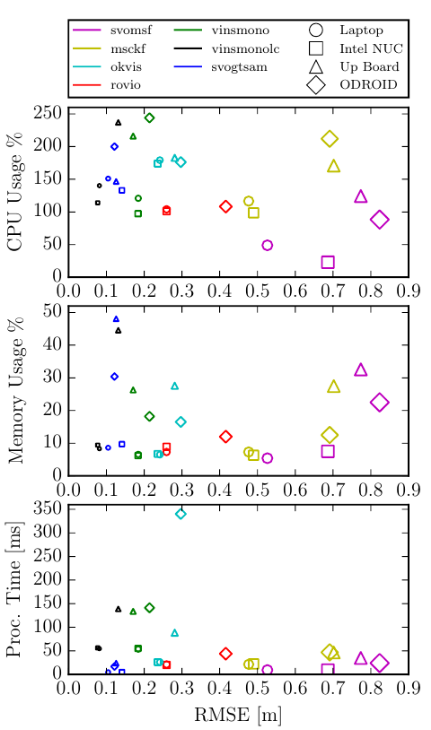
\includegraphics[width=0.6\textwidth]{4.png}    
\caption{VIO方案对比}
\label{img0}
\end{figure}
\indent 工业界,高巨创新MARK无人机采用的VIO(视觉惯性里程计)技术,革新定位方式,通过机身前端向下倾斜45°的鱼眼广角镜头与机身内
部IMU结合实现精准定位,可在室内无GPS的环境中飞行,实现MARK室内外来回自由穿梭,并且悬停更稳定。飞行器通过图像
比对进行定位导航,无需校准磁场便可直接起飞,也不受复杂磁场环境干扰,自动对下方地面障碍物或积水等,降低定位误差,
大幅提升降落精度。\\
\begin{figure}[H]
\centering
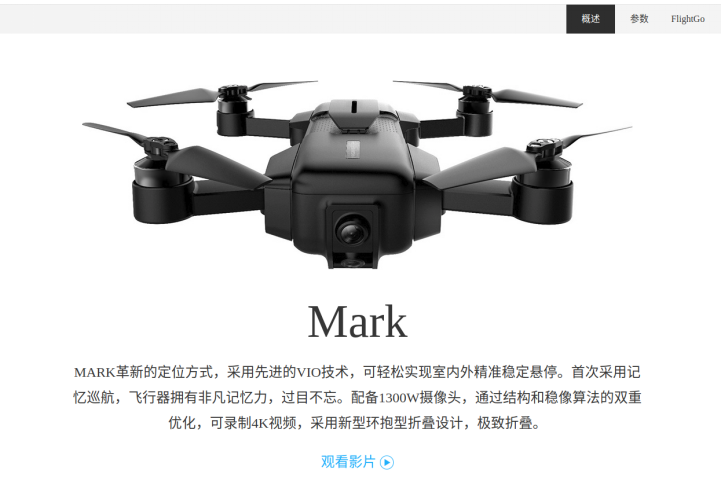
\includegraphics[width = .8\textwidth]{1.png}
\caption{VIO工业应用}
\end{figure}

\subsection{在学术界,VIO研究有哪些新进展?有没有将学习方法用到VIO中的例子?}
\indent VIO预积分技术极大推动了VIO的发展进程。IMU的数据通过积分,可以获取当前位姿(p位置,q四元数表达的姿态)、瞬时速度
等参数。在VINS中便使用了预积分技术。预积分是Christian Forster(SVO作者)在15年做的工作,发表在2015年的RSS(Robotics: Science and Systems)上。
预积分给出了一种比较优雅的,在SO(3)流形上处理IMU运动的方法,并给出了实现代码(gtsam中)。因此,了解预积分,会对VIO
的研究有重要的意义。\\
\indent 首次使用DL的框架解决VIO问题是VINet。传统VIO的框架一般可分为三个过程,基于图像序列的光流估计、基于惯
性数据的积分操作以及基于滤波和优化的运动融合。这种网络使用FlowNet来建模视觉运动特征,用LSTM来建模IMU的运动特
征,最后通过李群李代数中的SE(3)流行来建模位姿,用帧间堆叠的LSTM网络来预测位姿。同时,VINet在面对时间不同步和
外参标定不准确的多视觉惯导数据时,表现出了一定的优势。\\
\indent 最新论文Shamwell, E. Jared, et al. "Unsupervised Deep Visual-Inertial Odometry with Online 
Error Correction for RGB-D Imagery." IEEE transactions on pattern analysis and machine intelligence (2019).
学会了在没有惯性测量单元(IMU)内在参数或IMU和摄像机之间的外部校准的情况下执行视觉惯性里程计(VIO)。\\

\newpage
\section{编程验证题}
\subsection{代码}
% \begin{figure}[h]
% \centering
% 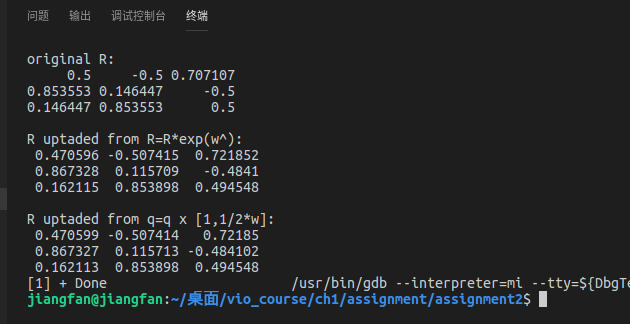
\includegraphics[width =0.6\textwidth]{2.png}
% \caption{代码截图}
% \end{figure}
\begin{lstlisting}[language={c++}]
    #include <iostream>
    #include <Eigen/Dense>
    
    using namespace std;
    using namespace Eigen;
    
    int main()
    {
        Eigen::Matrix3d R0=Eigen::AngleAxisd(M_PI/4,Eigen::Vector3d(1,0,0)).toRotationMatrix()
                        *Eigen::AngleAxisd(M_PI/4,Eigen::Vector3d(0,1,0)).toRotationMatrix()
                        *Eigen::AngleAxisd(M_PI/4,Eigen::Vector3d(0,0,1)).toRotationMatrix();
        cout<<"original R:"<<endl<<R0<<endl<<endl;
        Eigen::Vector3d omiga;
        omiga<<0.01,0.02,0.03;
    
        // update rotation matrix
        // compute exp(w_hat)
        double theta=sqrt(omiga(0)*omiga(0)+omiga(1)*omiga(1)+omiga(2)*omiga(2));
        Eigen::AngleAxisd w(theta,omiga/theta);
        Eigen::Matrix3d deltaR=w.toRotationMatrix();
        //cout<<"w_R:"<<deltaR<<endl;
        Eigen::Matrix3d Rnew;
        Rnew=R0*deltaR;
        cout<<"R uptaded from R=R*exp(w^):"<<endl<<Rnew<<endl;
    
        cout<<endl;
    
        // update quanternion
        Eigen::Quaterniond q(R0);
        Eigen::Quaterniond deltaq(1,0.5*omiga(0),0.5*omiga(1),0.5*omiga(2));
        //cout<<"deltaq:"<<deltaq.coeffs()<<endl;
        deltaq=deltaq.normalized();
        //cout<<"deltaq:"<<deltaq.coeffs()<<endl;
        //cout<<"q_R:"<<deltaq.toRotationMatrix()<<endl;
        Eigen::Quaterniond qnew;
        qnew=q*deltaq;
        qnew.normalized();-
        cout<<"R uptaded from q=q x [1,1/2*w]:"<<endl<<qnew.toRotationMatrix()<<endl;
        
        return 0;
    }
    
\end{lstlisting}

\subsection{运行结果截图}
\begin{figure}[h]
\centering
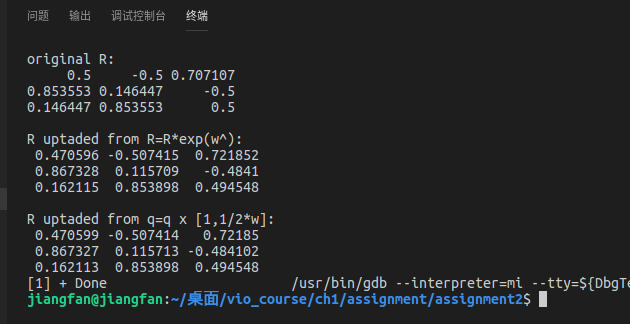
\includegraphics[width = 0.8\textwidth]{2.png}
\caption{运行结果截图}
\end{figure}
\indent 根据程序运行结果,可以发现使用李代数更新旋转矩阵和使用四元数更新四元数这两种方法得到的结果是非常接近的。

\newpage
\section{公式推导题}
\subsection{第一小题}
\begin{equation}
\begin{aligned}
\frac{d(R^{-1}p)}{dR}
&=\lim_{\phi \to 0}\frac{(Rexp(\phi^\wedge))^Tp-R^Tp}{\phi}\\
&=\lim_{\phi \to 0}\frac{(exp(\phi^\wedge))^TR^Tp-R^Tp}{\phi}\\
&=\lim_{\phi \to 0}\frac{(I+\phi^\wedge)^TR^Tp-R^Tp}{\phi}\\
&=\lim_{\phi \to 0}\frac{(\phi^\wedge)^TR^Tp}{\phi}\\
&=\lim_{\phi \to 0}\frac{(-\phi)^{\wedge}R^Tp}{\phi}\\
&=\lim_{\phi \to 0}\frac{(-R^Tp)^{\wedge}{(-\phi)}}{\phi}\\
&=(R^Tp)^\wedge
\end{aligned}
\end{equation}
\subsection{第二小题}
\begin{equation}
\begin{aligned}
\frac{dln({R_1}{R^{-1}_2})}{dR_2}
&=\lim_{\phi \to 0}\frac{{ln({R_1{{R_2exp({\phi^\wedge)}^T}})}-{ln({R_1R^T_2})}}}{\phi}\\
&=\lim_{\phi \to 0}\frac{ln(R_1(exp(\phi^\wedge))^TR^T_2)-{ln({R_1R^T_2})}}{\phi}\\
&=\lim_{\phi \to 0}\frac{{ln(R_1R^T_2R_2(exp(\phi^\wedge))^TR^T_2)}-{ln({R_1R^T_2})}}{\phi}\\
&=\lim_{\phi \to 0}\frac{ln(R_1R^T_2(R_2exp(\phi^\wedge)R^T_2)^T)-ln({R_1R^T_2})}{\phi}\\
&=\lim_{\phi \to 0}\frac{ln(R_1R^T_2(exp((R_2\phi)^\wedge))^T)-ln(R_1R^T_2)}{\phi}\\
&=\lim_{\phi \to 0}\frac{ln(R_1R^T_2exp((-R_2\phi)^\wedge))-ln(R_1R^T_2)}{\phi}\\
&=\lim_{\phi \to 0}\frac{ln(R_1R^T)+J^{-1}_r(-R_2\phi)-ln(R_1R^T_2)}{\phi}\\
&=\lim_{\phi \to 0}\frac{-J^{-1}_r(R_2\phi)}{\phi}\\
&=-J^{-1}_r((ln(R_1R^{-1}_2))^\vee)R_2
\end{aligned}
\end{equation}

\newpage
\begin{thebibliography}{1}
\bibitem{Gui}  Jianjun Gui, Dongbing Gu, Sen Wang , Huosheng Hu . A review of
visual inertial odometry from filtering and optimisation perspectives[J], Advanced Robotics, 29:20,
1289-1301,2015.
\bibitem{J} J. Delmerico. A Benchmark Comparison of Monocular Visual-Inertial Odometry Algorithms for Flying Robots[J],ICRA. 2018.
\bibitem{Joan} Joan Solà.Quaternion kinematics for the error-state Kalman filter[M], 2017.
\bibitem{gao} 高翔,视觉SLAM十四讲[M],北京:电子工业出版社,2017.
\bibitem{Shamwell}Shamwell, E. Jared, et al. "Unsupervised Deep Visual-Inertial Odometry with Online 
Error Correction for RGB-D Imagery." IEEE transactions on pattern analysis and machine intelligence (2019).
\end{thebibliography}

\end{document}

